\documentclass{beamer}
\usepackage{../preamble/custom}

\setbeamertemplate{bibliography item}[text]

\title{Maximal repetition \& ``Runs'' conjecture}
\author{Riccardo Lo Iacono \\ \footnotesize{Docente: Gabriele Fici}}
\begin{document}
    \begin{frame}
        \maketitle
    \end{frame}

    \begin{frame}{Notazione}
        \begin{enumerate}
            \item \(\Sigma\) è un alfabeto ordinato e finito di simboli
            \item Un elemento \(S \in \Sigma^{*}\) è detto stringa,
                la cui lunghezza è denotata da \(\abs{S}\)
            \item Per ogni i, \(1 \le i \le n = \abs{S}\), 
                S[i] indica l'i-esimo carattere in S.
            \item Per ogni i, j, \(1 \le i \le j \le n = \abs{S}\),
                S[i, j] indica la sottostringa compresa tra le 
                posizioni i e j, 
        \end{enumerate}
    \end{frame}

    \begin{frame}{Periodo ed esponente}
        \textbf{Definizione: } Data S una stringa,
        si definisce \emph{periodo} un intero \(p \ge 1\)
        tale che S[i] = S[i + p], \(\forall i = 1, \ldots, \abs{S} - p\)

        \textbf{Definizione: } Si definisce \emph{esponente} \(\exp\)
        il rapporto tra la lunghezza di S e del suo più piccolo periodo.
    \end{frame}

    \begin{frame}{Ripetizioni massimali}
        \textbf{Definizione: } Una coppia (i, j) è detta ripetizione massimale
        (o run) di una stringa S, se \(\exp(S[i, j]) \ge 2p\) e la periodicità
        non può essere estesa ne a destra ne a sinistra.
    \end{frame}

    \begin{frame}{Un esempio}
        Sia considerata la stringa \(S = babbabbababbabbabc\); questa contiene nove 
        run, mostrati in \emph{Figura \ref{fig:1}}.

        \begin{figure}[!h]
            \centering
            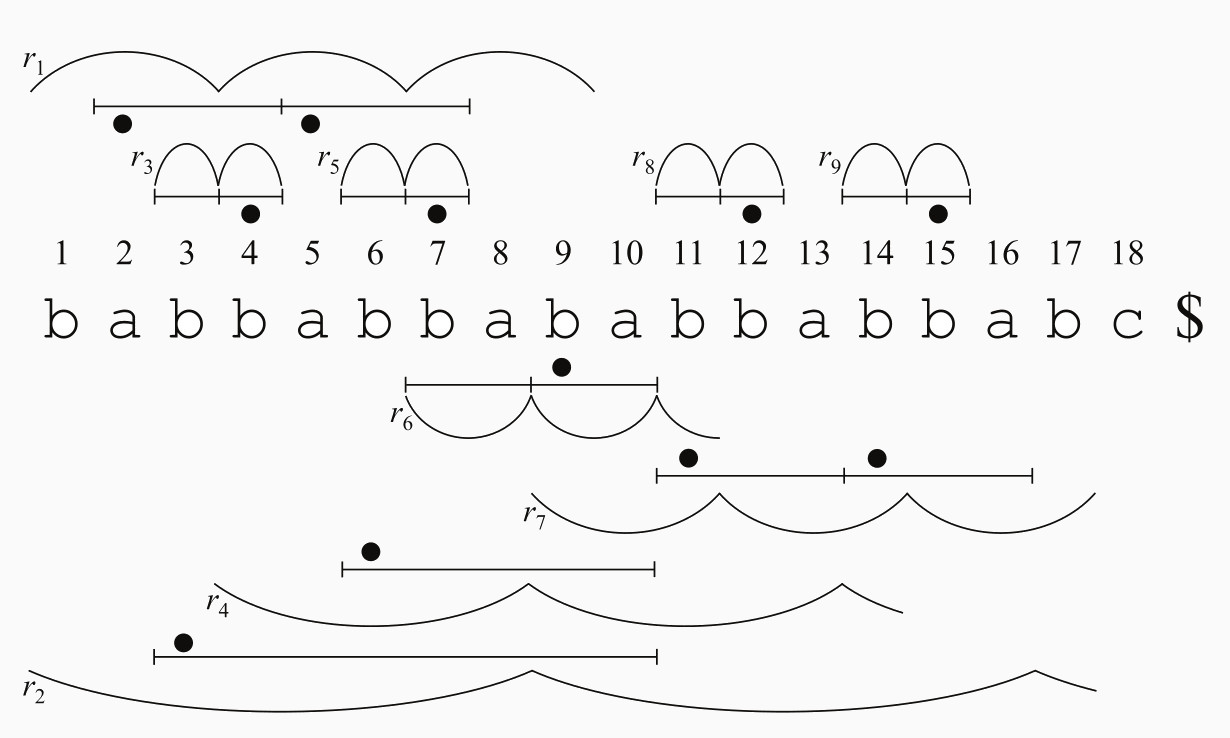
\includegraphics[scale = .85]{../Extra/run example.jpg}
            \caption{Illustrazione dei run nella stringa S = babbabbababbabbabc.}
            \label{fig:1}
        \end{figure}
    \end{frame}

    \begin{frame}{Background storico}

        Sia \(\rho(S)\) il numero dei run in una stringa S.

        \emph{Kolpakov \emph{e} Kucherov}\footnotemark[1]
        dimostrano che \(\rho(S) = \bigO{|S|}\).
        \vskip 10pt
        \textbf{Congettura (Runs conjecture):} \(\rho (S) < |S|\) per ogni stringa S.

        \footnotetext[1]{R. M. KUCHEROV {\footnotesize AND} G. KOLPAKOV,
                 \emph{Finding maximal repetitions in a word in linear time. FOCS, 1999}
         }
    \end{frame}

    \begin{frame}{Punti chiave della discussione}
        \begin{enumerate}
            \item Dimostrazione della runs conjecture.
            \item Applicazione della soluzione algoritmica.
        \end{enumerate}
    \end{frame}

    \begin{frame}{Lyndon words}

        Sia \(\prec\) l'ordine totale definito su \(\Sigma\),
        e si indichi con lo stesso l'ordine indotto su \(\Sigma^{*}\).
        
        Assunto \(\prec \text{ su } \Sigma\), si può definire \(\tilde{\prec}\)
        l'ordine rovesciato. Ossia, un'ordine tale per cui presi \(a, b \in \Sigma\),
        se 
        \[
            a \prec b \implies b \ \tilde{\prec} \ a
        \]

        Siano \(\prec_{0}, \prec_{1}\) rispettivamente l'ordine indotto su 
        \(\Sigma^{*}\) e l'ordine rovesciato.

    \end{frame}
    \begin{frame}
        Data S una stringa e un indice i, \(1 \le i \le n\),
        la stringa S[i, n]S[1, i] è detta \emph{shift ciclico} di S 
        (se i > 1 \emph{shift ciclico non banale}).

        \textbf{Definizione (Lyndon word): } 
        Una stringa \(S \in \Sigma^{*}, S \ne \varepsilon\),
        è detta Lyndon word se S è minore di ogni suo shift ciclico non banale.
    \end{frame}
    \begin{frame}{La ``Runs'' conjecture}
        \textbf{Congettura: } \(\rho(S) < \abs{S}\), per ogni stringa S.

        \textbf{Dimostrazione: } Sia S una stringa di lunghezza n,
        e sia (i, j), \(0 \le i < j < n\), un suo run con periodo p minore.

        Se j + 1 < n, ed inoltre S[j - p + 1] \(\prec_{0}\) S[j + 1],
        al run si assegna un indice k tale per cui S[k, j] è il \emph{longest proper suffisso}
        di S[i, j]. Viceversa k definisce il più lungo suffisso per \(\prec_{1}\).

        Si noti che se k > i allora k > 0, e S[k, j] contiene un intero periodo del run.
        Inoltre, S[k, k + p - 1] è il più lungo coniugato di S[i ,i + p - 1]
        rispetto i due ordini. Ciò implica l'essere \emph{border-free} % Che si intende?
        che è una proprietà nota delle Lyndon word.
    \end{frame}
    \begin{frame}
        Si intende dunque dimostrare che ogni k > 0 è posizione iniziale 
        di al più un solo \emph{longest proper suffix} in un run.

        Siano quindi considerati due run: (i, j) e (k, l) rispettivamente
        un p-run e un q-run. Inoltre, sia assunto per assurdo che 
        i loro longest proper suffix condividano la stessa posizione iniziale k.

        Poichè run distinti non possono avere uno stesso periodo si può assumere
        \(p \ne q\).
    \end{frame}
    \begin{frame}
        \begin{enumerate}
            \item j = l, ma allora S[k, j] = S[k, l].
                Assumendo per esempio p < q, S[k, k + q - 1] ha periodo p,
                ma allora questa non è border-free, che è una contraddizione.

            \item sia j < l, ragionamento analogo vale nel caso j > l, 
                inoltre siano i suffissi i più lunghi rispetto un stesso ordine.
                Posto d = S[j + 1], carattere successivo il p-run, 
                per definizione si ha S[j - p + 1] \(\prec\) d. 
                Inoltre, S[k, k - p + 1] \(\prec\) S[k, j - p]d. 
                Ma da ciò segue che S[k, l - 1] non è massimale come supposto,
                poichè S[i + p, j] è fattore del q-run.
        \end{enumerate}
    \end{frame}
    \begin{frame}
        \begin{enumerate}
            \item [3.] \(j \ne l\) e i suffissi risultano essere massimali secondo ordini diversi.
                Senza perdita di generalita sia p < q e il suffisso del p-run
                sia massimale rispetto \(\prec_{0}\).
                Poichè q > 1, si hanno S[k + q - 1] \(\prec_{0}\) S[k] e 
                S[k + q - 1] \(\prec_{1}\) S[k  - 1], da cui S[k - 1] \(\prec_{0}\) S[k].
                Si ha però che p \(\not\ge\) 1 (S[k] \(\prec_{0}\) S[k - 1]) 
                e p \(\ne\) 1 (S[k - 1] = S[k]). Da cui un'altra contraddizione.
        \end{enumerate}

        Ciò conclude la dimostrazione, 
        mostrando come il numero di run non possa essere superiore agli n - 1 
        potenziali valori di k.
    \end{frame}
\end{document}
